\documentclass{article}

\PassOptionsToPackage{numbers,sort&compress}{natbib}
\usepackage[preprint]{neurips_2024}

\usepackage[utf8]{inputenc}
\usepackage[T1]{fontenc}
\usepackage[colorlinks=true,linkcolor=blue,citecolor=blue,urlcolor=blue]{hyperref}
\usepackage{url}
\usepackage{booktabs}
\usepackage{amsmath,amssymb}
\usepackage{graphicx}
\usepackage{microtype}
\usepackage{xcolor}
\usepackage{multirow}

\newcommand{\Tc}{T_{\mathrm{c}}}
\newcommand{\Tcad}{T_{\mathrm{c,AD}}}
\newcommand{\Eform}{E_{\mathrm{form}}}
\newcommand{\Ehull}{E_{\mathrm{hull}}}
\newcommand{\todo}[1]{\textcolor{red}{[TODO: #1]}}

\title{Preference and Reward Optimization for Superconductor Crystal Diffusion}

\author{
  Wenhe Zhang \\
  Yale University \\
  \texttt{wenhe.zhang@yale.edu}
  \And
  Jeffrey Wei \\
  Yale University \\
  \texttt{jeffrey.wei@yale.edu}
}

\begin{document}
\maketitle

\begin{abstract}
Generative crystal diffusion models can propose large numbers of candidate materials, but their practical usefulness depends on how many generated structures pass downstream physical screens. We study post-training methods for the GuidedMatDiffusion superconductor generator, a property-conditioned DiffCSP model trained to generate periodic crystal structures for target superconducting critical temperature. Our project asks whether preference/reward optimization can shift the generator toward candidates with better superconductivity and screening properties while preserving structural validity. Wenhe Zhang implemented and evaluated a Group Relative Policy Optimization (GRPO) post-training pipeline using BEE-NET, MEGNet, and optional M3GNet/proxy rewards. Jeffrey Wei investigates Direct Preference Optimization (DPO) for the same generator. In a deadline-scale GRPO experiment with 150 updates, the policy preserved validity and diversity, improved mean absolute target-temperature error from 5.06 K to 4.82 K, improved mean target uplift by 2.53 K over the frozen reference policy, and increased metallic pass rate from 0.75 to 0.91, though cheap-filter pass rate decreased from 0.59 to 0.50. These results suggest that reward-based post-training can measurably change the diffusion generator in the desired direction, but longer training and stronger stability rewards are needed for robust screening gains.
\end{abstract}

\section{Introduction and Problem Definition}
Superconductors are materials with zero electrical resistance below a critical temperature $\Tc$, with potential applications in energy transmission, high-field magnets, sensors, and quantum devices. Discovering new superconductors remains expensive because candidate structures must satisfy several coupled constraints: they should be chemically plausible, metallic, thermodynamically or dynamically stable, and have favorable electron--phonon properties. Recent guided diffusion models for crystals can generate many plausible candidates, but generation is still followed by a costly filtering pipeline, and most samples may fail at least one screening stage.

We address the inverse design problem: given a desired superconducting target, generate novel periodic crystal structures that have high expected downstream screening reward. The base model is a conditional crystal diffusion model that learns a distribution over lattice matrices, fractional coordinates, and atom types for periodic crystals conditioned on a scalar target property $\Tcad$. Rather than only changing the classifier-free guidance weight at inference time, our project tests whether post-training objectives can update the generator itself.

Our team studies two complementary approaches. Wenhe Zhang implemented GRPO fine-tuning of the diffusion sampler using grouped rollouts and surrogate rewards. Jeffrey Wei is responsible for a DPO-style preference fine-tuning method. Together, these methods ask whether reward/preference optimization can improve hit rate and target alignment without collapsing validity or diversity.

\section{Dataset}
\paragraph{Data source.}
We use the processed superconductivity dataset released with GuidedMatDiffusion, \texttt{supccomb\_12}. The dataset combines superconducting candidate structures and electron--phonon-derived labels from prior high-throughput superconductivity studies. Each sample is a periodic crystal structure paired with a target property \texttt{tcad}, the Allen--Dynes corrected critical temperature estimate. The local split used by the codebase contains \texttt{train.csv}, \texttt{val.csv}, and \texttt{test.csv}; the training CSV is also used to sample target prompts for GRPO.

\paragraph{Graph representation.}
Each structure is represented as a periodic atom graph. Nodes are atoms with atomic-number attributes. Edges are produced by CrystalNN under periodic boundary conditions and include periodic image offsets. The diffusion model operates on lattice parameters, fractional coordinates, and atom types rather than ordinary molecular graphs; however, PyTorch Geometric batching is used throughout preprocessing and training.

\paragraph{EDA summary.}
Table~\ref{tab:eda} summarizes the processed dataset statistics from our proposal analysis. The dataset is small relative to large materials corpora and has a strongly right-skewed $\Tcad$ distribution, making high-$\Tc$ generation a low-yield target. The graph density is high because unit cells are small and CrystalNN often connects many periodic neighbors.

\begin{table}[t]
\centering
\small
\setlength{\tabcolsep}{4pt}
\begin{tabular}{@{}ll@{}}
\toprule
\textbf{Statistic} & \textbf{Value} \\
\midrule
Total samples & 7,183 \\
Split sizes (train / validation / test) & 5,746 / 718 / 719 \\
Max atoms per cell & 12 \\
Nodes per graph & $4.914 \pm 1.865$ \\
Undirected edges per graph & $8.456 \pm 8.672$ \\
Graph density & $0.774 \pm 0.193$ \\
Average clustering coefficient & $0.445 \pm 0.464$ \\
Mean node degree & $2.964 \pm 1.524$ \\
Unique elements per graph & $2.903 \pm 0.585$ \\
$\Tcad$ mean $\pm$ std & $3.596 \pm 5.215$ K \\
$\Tcad$ quartiles & $0.052$ / $0.993$ / $5.482$ K \\
Fraction with $\Tcad > 5$ K / $10$ K / $20$ K & $26.52\%$ / $12.53\%$ / $1.56\%$ \\
\bottomrule
\end{tabular}
\caption{EDA summary for \texttt{supccomb\_12}. Graph metrics are computed after collapsing duplicated directed CrystalNN edges.}
\label{tab:eda}
\end{table}

\begin{figure}[t]
  \centering
  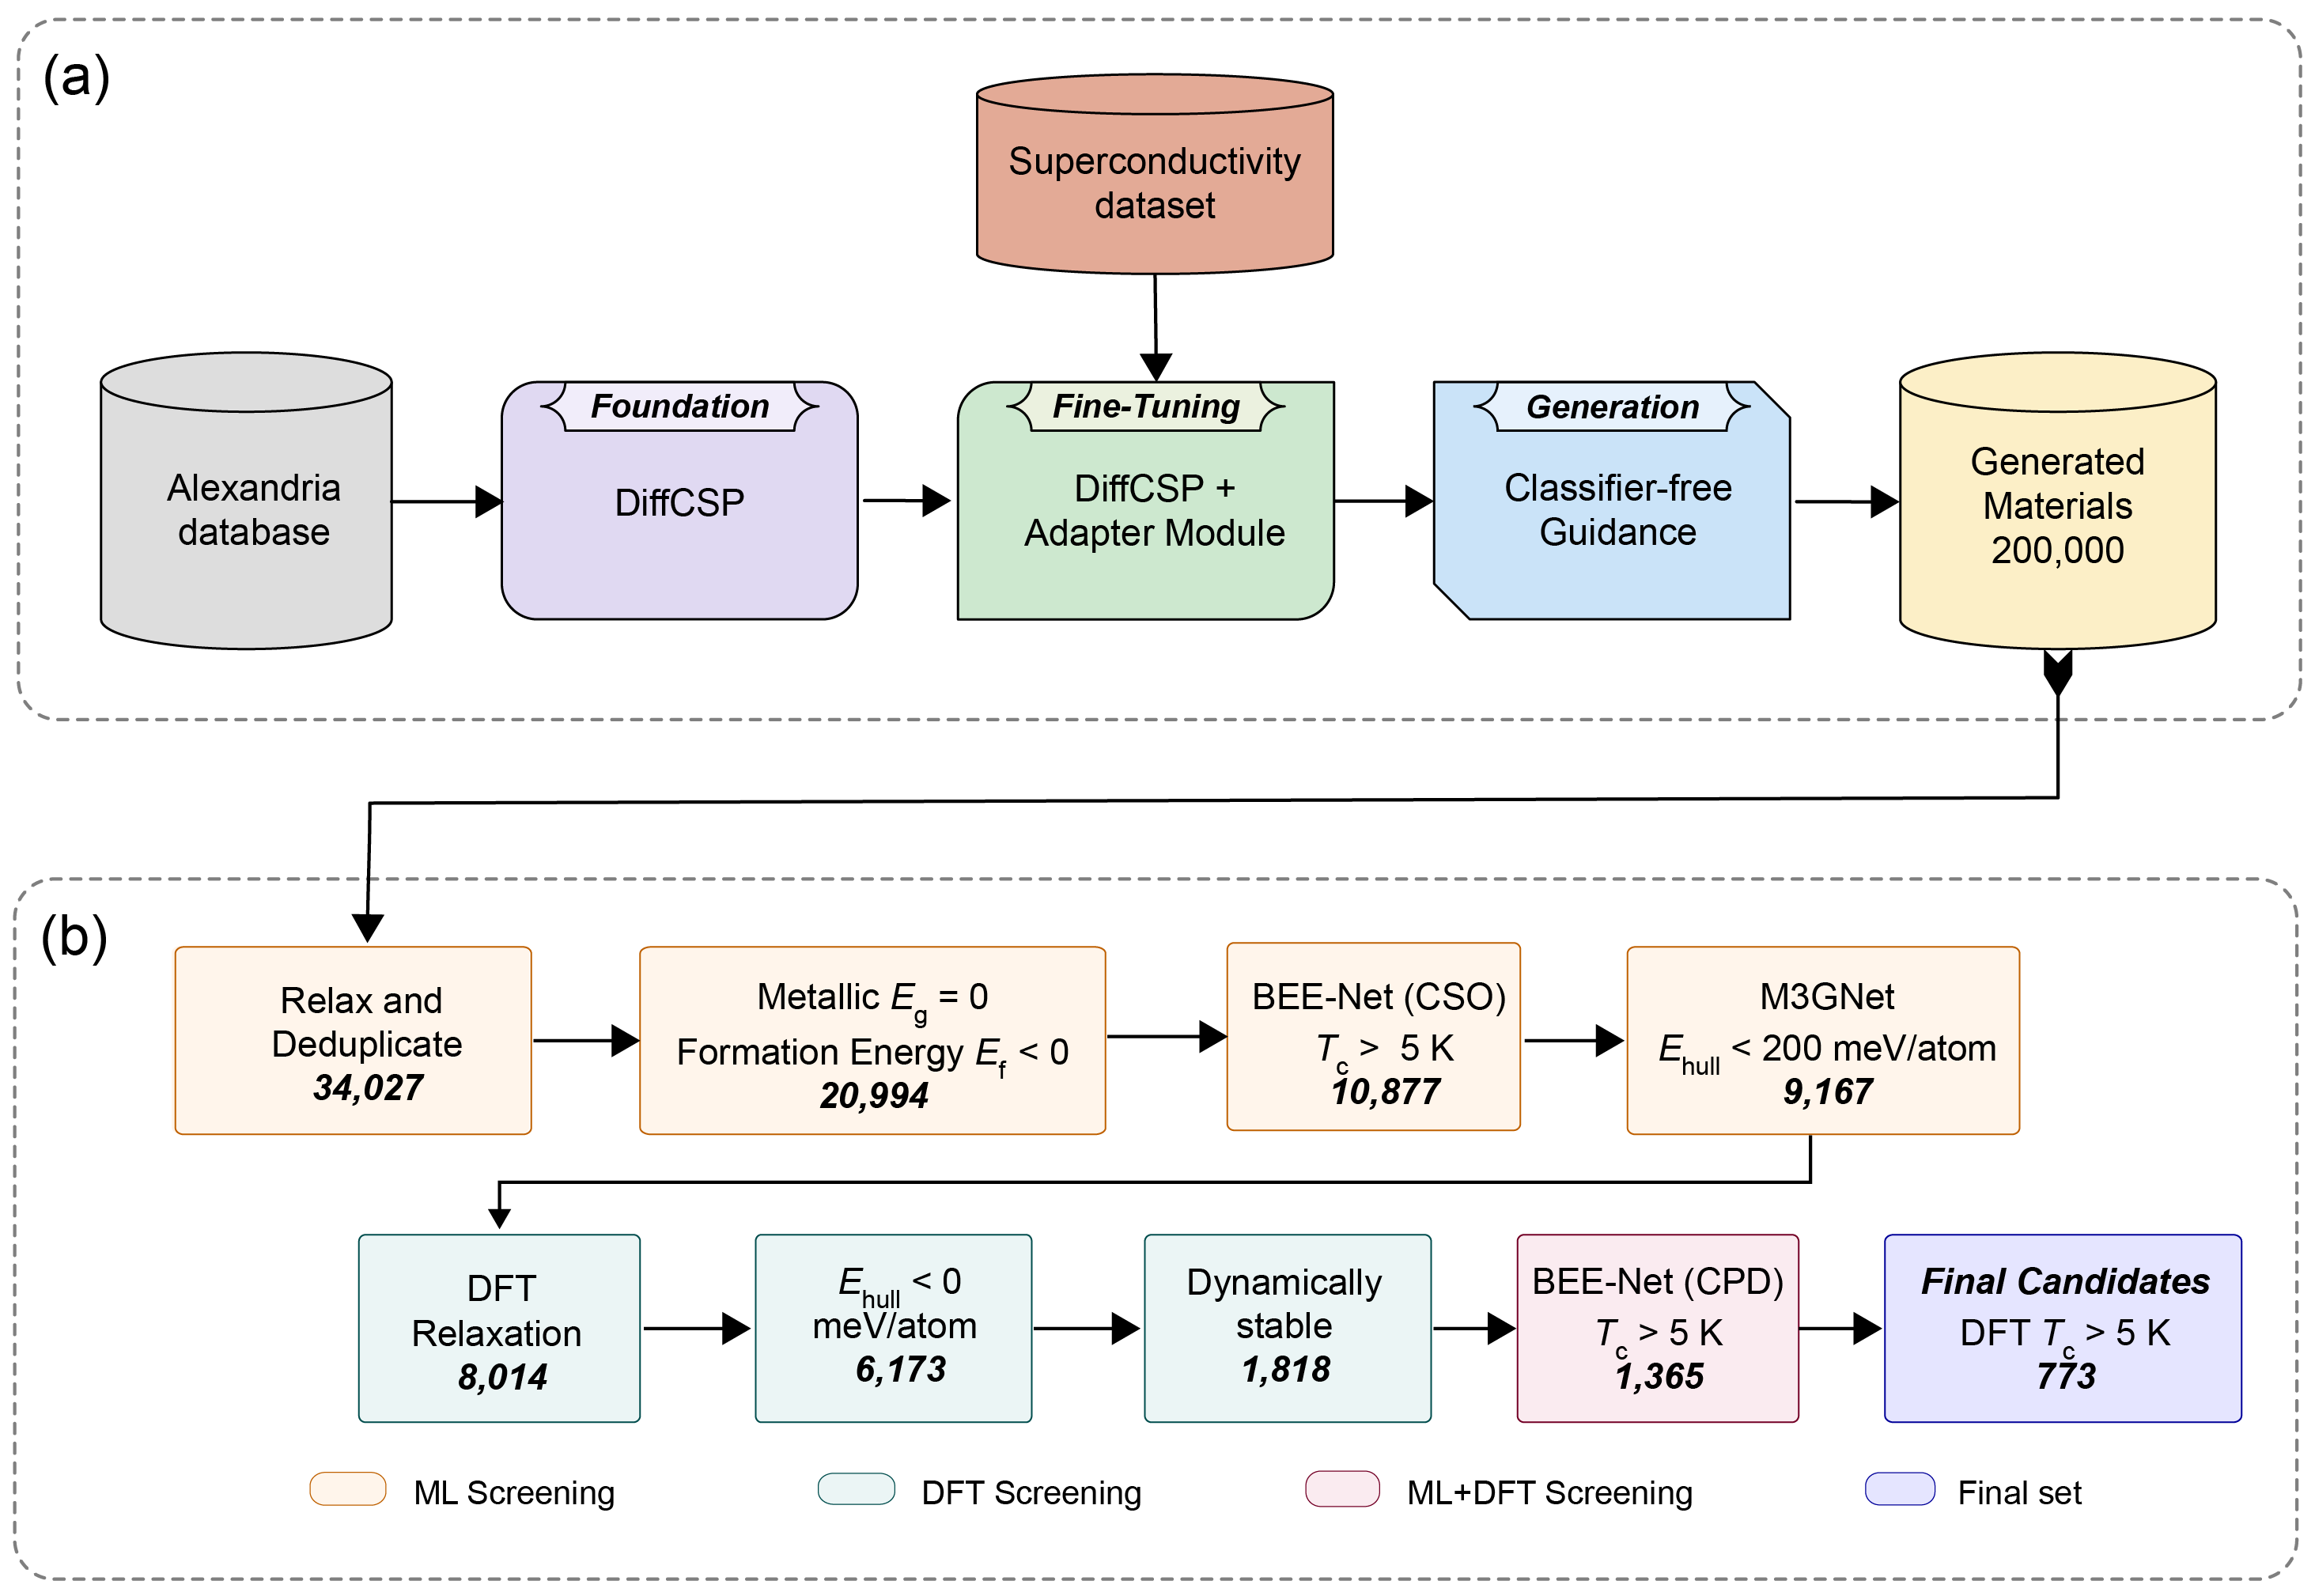
\includegraphics[width=0.92\linewidth]{fig/workflow.png}
  \caption{GuidedMatDiffusion workflow. Our project modifies the generation stage by adding GRPO/DPO post-training before downstream screening, rather than relying only on classifier-free guidance and post-hoc filtering.}
  \label{fig:workflow}
\end{figure}

\section{Related Work}
\paragraph{Crystal diffusion.}
DiffCSP introduced joint equivariant diffusion over crystal lattices and fractional coordinates, making it a natural backbone for periodic crystal generation and structure prediction~\citep{jiao2023diffcsp}. GuidedMatDiffusion builds on DiffCSP by pretraining on Alexandria and fine-tuning on superconductivity data, then applying classifier-free guidance for conditional superconductor generation~\citep{prakash2025guidedmatdiffusion}. Our project keeps this backbone fixed as the base generator and studies post-training methods for improving the sampling distribution.

\paragraph{Surrogate screening models.}
MEGNet provides graph-network predictors for materials properties such as band gap and formation energy~\citep{chen2019megnet}. M3GNet extends graph neural networks into universal interatomic potentials for relaxation and stability estimation~\citep{chen2022m3gnet}. BEE-NET and related AI-accelerated superconductivity workflows provide fast structure-based approximations to electron--phonon superconductivity quantities~\citep{gibson2025workflow}. These models are imperfect substitutes for DFT, but they make reward-based optimization feasible inside a class-project compute budget.

\paragraph{Preference and reward optimization.}
Classifier-free guidance changes samples at inference time but does not change the generator parameters~\citep{ho2022classifierfree}. DPO directly optimizes models from pairwise preferences without an explicit reward model~\citep{rafailov2023dpo}. GRPO is a PPO-style grouped policy optimization method that normalizes rewards within sampled groups, avoiding a learned value model in some settings~\citep{shao2024deepseekmath}. We adapt this idea to diffusion trajectories: multiple branches share a denoising prefix, receive reward scores, and update the diffusion policy using branch-relative advantages.

\section{Methodology}
\subsection{Base Model: GuidedMatDiffusion}
The base generator is the released GuidedMatDiffusion checkpoint for \texttt{supccomb\_12}. It uses a CSPNet denoiser with message passing over periodic atom graphs. During training, lattice matrices, fractional coordinates, and atom-type one-hot vectors are noised, and the model predicts denoising targets. Property conditioning is injected through adapter modules that embed the target \texttt{tcad}; at inference time, classifier-free guidance combines conditional and unconditional predictions.

\subsection{Wenhe Zhang: GRPO Fine-Tuning}
\paragraph{Rollout construction.}
For each GRPO group, we sample a target $\Tcad$ prompt from the training distribution with a bias toward the upper quartile. We sample an atom count from the empirical \texttt{supccomb\_12} atom-count prior. The policy first runs a shared diffusion prefix, then branches into $K$ stochastic completions. This creates comparable candidates conditioned on the same target and prefix.

\paragraph{Reward model.}
Each branch is scored by a composite surrogate reward. BEE-NET estimates superconductivity quantities and provides dense shaping toward the requested $\Tcad$:
\begin{equation}
\phi_{\mathrm{BEE}}(x,y) =
-\frac{|\widehat{\Tcad}(x)-y|}{\sigma_{\Tcad}}
+0.25\frac{\max(\widehat{\Tcad}(x)-y,0)}{\sigma_{\Tcad}} .
\end{equation}
MEGNet provides terminal rewards for metallicity and formation energy:
\begin{equation}
R_{\mathrm{MEG}}(x)
=0.5\mathbf{1}\{\widehat{E}_g(x)\leq 0.05\}
-0.5\,\mathrm{softplus}\!\left(\widehat{E}_{\mathrm{form}}(x)/0.05\right).
\end{equation}
The code also supports M3GNet relaxation rewards and offline proxy rewards, but these were disabled in the reported deadline run to keep runtime manageable.

\paragraph{Policy objective.}
For each branch, we recompute per-step diffusion log probabilities under the current policy and a frozen reference policy. Branch rewards are normalized within the group to form advantages. The policy loss uses a clipped ratio objective with reference KL:
\begin{equation}
\mathcal{L}_{\mathrm{GRPO}}
=-\mathbb{E}_{b,t}\left[
\min(r_{b,t}A_{b,t},
\mathrm{clip}(r_{b,t},1-\epsilon,1+\epsilon)A_{b,t})
\right]
\;+\;\beta_{\mathrm{KL}}\,
\mathbb{E}_{b,t}\left[\log p_\theta-\log p_{\mathrm{ref}}\right].
\end{equation}
This update is intentionally conservative: it tries to improve reward while staying near the pretrained structural prior.

\paragraph{Implementation contributions.}
I added the GRPO entry point, prompt sampler, reward manager, and trainer in \texttt{diffcsp/run\_rl.py} and \texttt{diffcsp/rl/}. I modified the diffusion sampler to expose shared-prefix branch rollouts and per-step log probabilities. I integrated BEE-NET and MEGNet smoke tests, fixed nested Hydra loading for checkpoint configs, added dtype hardening after BEE-NET changed the global Torch default dtype, clamped wrapped-normal log-probabilities to avoid NaNs at deterministic final diffusion steps, and added \texttt{train\_progress.jsonl} logging for reproducibility.

\subsection{Jeffrey Wei: DPO Fine-Tuning}
\todo{Jeffrey: describe your DPO data construction, preference labels, objective, implementation files, and how it differs from GRPO. Include the DPO equation and any details about which parameters/layers were updated.}

\section{Experiments and Results}
\subsection{Experimental Setup}
\paragraph{Baselines.}
The primary baseline is the frozen GuidedMatDiffusion \texttt{supccomb\_12} checkpoint evaluated under the same target prompts and guidance-weight grid. We compare the GRPO policy against the frozen reference at guidance weights $\{0.5,1.0,2.0\}$.

\paragraph{Metrics.}
We report mean absolute $\Tcad$ error against the requested target, mean $\Tcad$ uplift, metallic pass rate, negative-formation-energy pass rate, cheap-filter pass rate (valid, metallic, and negative formation energy), invalid rate, and duplicate rate. These metrics match the project goal: reward optimization should improve target satisfaction and screening proxies while preserving physical validity and diversity.

\paragraph{Hardware and runtime.}
Experiments were run on a cluster node with an NVIDIA H200 GPU. BEE-NET was run on CUDA; MEGNet used TensorFlow CPU fallback because its CUDA 11 runtime libraries were unavailable in the environment. The final GRPO report run used 150 updates and completed in roughly 1.5 hours including final evaluation.

\paragraph{GRPO hyperparameters.}
The final report run used \texttt{max\_updates=150}, \texttt{num\_groups\_per\_update=1}, \texttt{num\_branches=2}, \texttt{prefix\_t=50}, \texttt{reward\_interval=25}, Adam learning rate $5\times 10^{-7}$, clipping $\epsilon=0.02$, KL coefficient $0.05$, gradient norm clipping $1.0$, BEE-NET ensemble size $1$, and M3GNet/proxy rewards disabled. Final evaluation used 32 prompts and compared policy vs. reference.

\subsection{Quantitative Results}
Table~\ref{tab:grpo_results} shows the final 150-update GRPO run. The GRPO policy's best deployment guide weight was $2.0$, while the reference's best guide weight was $0.5$ under the composite selection rule.

\begin{table}[t]
\centering
\small
\setlength{\tabcolsep}{4pt}
\begin{tabular}{@{}lccc@{}}
\toprule
\textbf{Metric} & \textbf{GRPO policy} & \textbf{Frozen reference} & \textbf{Delta} \\
\midrule
Best guide weight & 2.0 & 0.5 & -- \\
Mean absolute $\Tcad$ error (K) & 4.821 & 5.061 & $-0.241$ \\
Mean $\Tcad$ uplift (K) & $-1.709$ & $-4.239$ & $+2.530$ \\
Metallic pass rate & 0.906 & 0.750 & $+0.156$ \\
Negative $\Eform$ pass rate & 0.531 & 0.812 & $-0.281$ \\
Cheap-filter pass rate & 0.500 & 0.594 & $-0.094$ \\
Invalid rate & 0.000 & 0.000 & 0.000 \\
Duplicate rate & 0.000 & 0.000 & 0.000 \\
Composite score & $-0.503$ & $-0.576$ & $+0.073$ \\
\bottomrule
\end{tabular}
\caption{Final GRPO report-run metrics at update 150, compared with the frozen reference policy on the same 32-prompt evaluation protocol.}
\label{tab:grpo_results}
\end{table}

\begin{table}[t]
\centering
\small
\setlength{\tabcolsep}{4pt}
\begin{tabular}{@{}lccccccc@{}}
\toprule
\textbf{Model} & \textbf{$w$} & \textbf{Abs. err.} & \textbf{Uplift} & \textbf{Metal} & \textbf{Neg. $\Eform$} & \textbf{Cheap} & \textbf{Invalid} \\
\midrule
GRPO & 0.5 & 5.242 & -3.411 & 0.594 & 0.688 & 0.312 & 0.000 \\
GRPO & 1.0 & 5.341 & -3.729 & 0.750 & 0.906 & 0.656 & 0.000 \\
GRPO & 2.0 & \textbf{4.821} & \textbf{-1.709} & \textbf{0.906} & 0.531 & 0.500 & 0.000 \\
Reference & 0.5 & 5.061 & -4.239 & 0.750 & 0.812 & 0.594 & 0.000 \\
Reference & 1.0 & 5.323 & -3.338 & 0.781 & 0.562 & 0.375 & 0.000 \\
Reference & 2.0 & 6.069 & -2.805 & 0.812 & 0.656 & 0.500 & 0.000 \\
\bottomrule
\end{tabular}
\caption{Guidance-weight ablation for the GRPO policy and frozen reference.}
\label{tab:guide_ablation}
\end{table}

\subsection{DPO Results}
\todo{Jeffrey: add your DPO quantitative table here. Suggested rows: frozen reference, DPO checkpoint, and optionally DPO at several guidance weights. Use the same metrics as Table~\ref{tab:grpo_results} so the comparison is clean.}

\subsection{Analysis and Discussion}
The GRPO run demonstrates that post-training can produce measurable movement in the intended direction without immediate collapse. The policy kept invalid rate and duplicate rate at zero, improved target-temperature error, and substantially improved $\Tcad$ uplift. It also improved metallic pass rate, suggesting the MEGNet band-gap component successfully influenced generation.

The main weakness is formation energy. The GRPO policy's negative-formation-energy pass rate fell relative to the reference, which lowered cheap-filter pass rate. This is plausible because the phase-A reward used only BEE-NET and MEGNet and did not include M3GNet relaxation/stability; moreover, the run was intentionally short and used a small BEE-NET ensemble for deadline reasons. A longer run or phase-B run with M3GNet subset rewards should better address stability, at the cost of significantly more compute.

We also observed important engineering failure modes. An early smoke run produced NaNs because the wrapped-normal log-probability evaluated a zero-sigma final diffusion step. We fixed this by clamping sigmas and adding a non-finite-loss guard. BEE-NET also changed the Torch default dtype to float64, causing dtype mismatches in the sampler; we fixed this by explicitly casting sampler tensors and property embeddings to the model dtype. These fixes were necessary for reproducible GRPO training.

\section{Conclusion}
We implemented a GRPO post-training pipeline for GuidedMatDiffusion and evaluated it on superconductor crystal generation. In a 150-update deadline-scale experiment, GRPO improved target-temperature alignment and metallicity while preserving validity and diversity. However, it did not improve the full cheap-filter pass rate because formation-energy pass rate decreased. This supports the hypothesis that reward optimization can steer the diffusion generator, but also shows that superconducting crystal design requires balancing multiple physical objectives. Future work should run longer phase-A training, enable M3GNet phase-B stability rewards, compare against DPO under matched budgets, and validate top candidates with more expensive physics calculations.

\section{Code Quality and Reproducibility}
The project code is organized as an extension of GuidedMatDiffusion. Core GRPO files are in \texttt{diffcsp/rl/} and \texttt{diffcsp/run\_rl.py}; sampler/log-probability changes are in \texttt{diffcsp/pl\_modules/}; smoke tests and reward utilities are in \texttt{scripts/}. To reproduce the GRPO result, use the \texttt{matdiff39} environment, install BEE-NET/MEGNet dependencies, set \texttt{PROJECT\_ROOT}, \texttt{HYDRA\_JOBS}, and \texttt{WABDB\_DIR}, then run:
\begin{verbatim}
python -m diffcsp.run_rl \
  expname=rl_grpo_report_150 \
  paths.policy_checkpoint=$PROJECT_ROOT/hf_models/superconductor_generator \
  grpo.schedule.max_updates=150 \
  grpo.sampling.num_groups_per_update=1 \
  grpo.sampling.num_branches=2 \
  grpo.sampling.prefix_t=50 \
  grpo.sampling.reward_interval=25 \
  grpo.eval.num_prompts=32 \
  grpo.eval.interval=150 \
  grpo.eval.compare_reference=true \
  grpo.checkpoint.interval=50 \
  grpo.rewards.bee.ensemble_size=1 \
  grpo.rewards.bee.device=cuda \
  grpo.rewards.m3gnet.enabled=false \
  grpo.rewards.proxies.enabled=false
\end{verbatim}
The final reported files are \texttt{rl\_update\_000150.pt} and \texttt{eval\_update\_000150.json} under \texttt{hydra\_jobs/singlerun/2026-05-02/rl\_grpo\_report\_150/}.

\begin{thebibliography}{10}

\bibitem{jiao2023diffcsp}
Rui Jiao, Wenbing Huang, Peijia Lin, Jiaqi Han, Pin Chen, Yutong Lu, and Yang Liu.
\newblock Crystal Structure Prediction by Joint Equivariant Diffusion.
\newblock In \emph{NeurIPS}, 2023.

\bibitem{prakash2025guidedmatdiffusion}
Pawan Prakash, Jason B. Gibson, Zhongwei Li, and others.
\newblock Guided Diffusion for the Discovery of New Superconductors.
\newblock \emph{arXiv preprint arXiv:2509.25186}, 2025.

\bibitem{chen2019megnet}
Chi Chen, Weike Ye, Yunxing Zuo, Chen Zheng, and Shyue Ping Ong.
\newblock Graph Networks as a Universal Machine Learning Framework for Molecules and Crystals.
\newblock \emph{Chemistry of Materials}, 2019.

\bibitem{chen2022m3gnet}
Chi Chen and Shyue Ping Ong.
\newblock A Universal Graph Deep Learning Interatomic Potential for the Periodic Table.
\newblock \emph{Nature Computational Science}, 2022.

\bibitem{gibson2025workflow}
Jason B. Gibson, Anubhav C. Hire, Peter M. Dee, Benjamin Geisler, Jung Soo Kim, Zhongwei Li, James J. Hamlin, Gregory R. Stewart, Peter J. Hirschfeld, and Richard G. Hennig.
\newblock Developing a Complete AI-Accelerated Workflow for Superconductor Discovery.
\newblock \emph{arXiv preprint arXiv:2503.20005}, 2025.

\bibitem{ho2022classifierfree}
Jonathan Ho and Tim Salimans.
\newblock Classifier-Free Diffusion Guidance.
\newblock \emph{arXiv preprint arXiv:2207.12598}, 2022.

\bibitem{rafailov2023dpo}
Rafael Rafailov, Archit Sharma, Eric Mitchell, Christopher D. Manning, Stefano Ermon, and Chelsea Finn.
\newblock Direct Preference Optimization: Your Language Model is Secretly a Reward Model.
\newblock In \emph{NeurIPS}, 2023.

\bibitem{shao2024deepseekmath}
Zhihong Shao, Peiyi Wang, Qihao Zhu, and others.
\newblock DeepSeekMath: Pushing the Limits of Mathematical Reasoning in Open Language Models.
\newblock \emph{arXiv preprint arXiv:2402.03300}, 2024.

\end{thebibliography}

\end{document}
